\chapter{Verifica pratica della robustezza su impianti incerti}

\section{Dieci impianti fisici comuni}
Per osservare come cambiano le prestazioni, estraiamo una volta
dieci quintuple di parametri con seed 20261101. La frequenza
naturale di ciascun drive cambia la zona in cui il comando è
attenuato, il ritardo ne cambia la fase e la massa $m_2$ modifica
la dinamica meccanica. Le frequenze sono fra 34 e 46 rad/s, i
ritardi fra 12 e 18 ms e la massa fra 0.72 e 0.88 kg. Lo
smorzamento dei drive resta a 0.8. Tutti i controllori sono
confrontati sulle stesse dieci quintuple e sul nominale, così
un caso sfavorevole può essere ripetuto con un altro controllore
senza cambiare la pianta. I valori sono salvati in
\texttt{parametri\_dieci\_impianti.csv}.
\begin{table}[htbp]\centering\small
\setlength{\tabcolsep}{4pt}
\begin{tabular}{lrrrrr}\toprule
Impianto & $\omega_{n1}$ & $\omega_{n2}$ & $\tau_{d1}$ & $\tau_{d2}$ & $m_2$\\\midrule
1 & \num{40.86} & \num{39.09} & \num{15.03} & \num{12.08} & \num{0.7793}\\
2 & \num{44.11} & \num{42.51} & \num{17.78} & \num{17.49} & \num{0.7559}\\
3 & \num{39.15} & \num{35.1} & \num{16.16} & \num{17.09} & \num{0.8014}\\
4 & \num{35.72} & \num{38.63} & \num{14.81} & \num{12.49} & \num{0.8038}\\
5 & \num{41.49} & \num{42.74} & \num{15.19} & \num{17.38} & \num{0.8181}\\
6 & \num{42.38} & \num{45.67} & \num{14.26} & \num{15.62} & \num{0.7903}\\
7 & \num{45.66} & \num{38.28} & \num{14.66} & \num{14.52} & \num{0.8205}\\
8 & \num{44.33} & \num{43.17} & \num{16.33} & \num{13.77} & \num{0.845}\\
9 & \num{45.23} & \num{41.22} & \num{14.36} & \num{13.02} & \num{0.7454}\\
10 & \num{44.54} & \num{34.26} & \num{14.49} & \num{17.23} & \num{0.8613}\\
\bottomrule\end{tabular}
\caption{Dieci impianti fisici comuni, seed 20261101. Frequenze in rad/s, ritardi in ms e massa in kg; smorzamento 0.8 noto.}
\end{table}


\section{Le rappresentazioni A e B sugli stessi campioni}
In A le frequenze, i ritardi e la massa entrano direttamente
come parametri fisici. In B il drive nominale riceve una
correzione dinamica additiva: il peso $W_A$ scala lo
scostamento possibile con la frequenza e una perturbazione
normalizzata ne specifica la dinamica. La massa $m_2$ resta
un parametro meccanico in entrambe.

Per ciascuno dei dieci impianti la perturbazione additiva
che ricostruisce il drive è la differenza rispetto al nominale
divisa per $W_A$. È stata controllata per stabilità, proprietà
e norma. Il massimo errore relativo di ricostruzione A/B è
\FinErroreAB. A controllore fissato le risposte dei due modelli
allo stesso campione coincidono entro questa precisione di
rappresentazione. B ammette anche dinamiche senza una
corrispondente coppia fisica di frequenza e ritardo, e la
copertura dell'intero box A resta da dimostrare. Il confronto
dei margini del Capitolo 9 valuta l'effetto di queste differenze
sull'intera famiglia dichiarata.

\section{Stabilità interna e tracking}
Prima di misurare il tracking si controllano tutti i poli
della chiusura. Un polo con parte reale positiva fa crescere
un modo interno, anche quando l'uscita di una certa prova
lo mostra poco. I casi instabili restano nel conteggio
(Tabella~\ref{tab:impianti-comuni}); i massimi di errore e
comando usano soltanto i casi stabili.

\begin{table}[htbp]\centering\small
\setlength{\tabcolsep}{4pt}
\begin{tabular}{lrrrr}\toprule
Controllore & Stabili & Errore DC [\%] & Picco u [N m] & Picco $q_d$ [$^\circ$]\\\midrule
LQG & 10/10 & \num{6.763} & \num{4.832} & \num{9.218}\\
LQGI & 10/10 & 0 & \num{0.9876} & \num{7.584}\\
Hinf1 & 10/10 & \num{15.54} & \num{14.74} & \num{14.63}\\
Hinf2 & 4/10 & \num{0.1643} & \num{1.001} & \num{2.717}\\
PID & 7/10 & 0 & \num{3.946} & \num{12.54}\\
Mu\_A & 10/10 & \num{99.8} & \num{0.001168} & \num{7.992}\\
Mu\_B & 10/10 & \num{22.36} & \num{0.8511} & \num{8.136}\\
\bottomrule\end{tabular}
\caption{Dieci impianti comuni: massimi sui soli casi stabili. Errore DC relativo e coppia link di 0.5 N m.}
\end{table}


Hinf2 resta stabile in \FinHinfTwoStable/10 campioni e PID in
\FinPIDStable/10. Il basso errore DC riportato per Hinf2
riguarda quindi un solo impianto incerto stabile. LQG, LQGI,
Hinf1, Mu\_A e Mu\_B sono stabili in tutti e dieci.
LQGI conserva un errore DC praticamente nullo nei campioni,
mentre il massimo di LQG sale al 5.41\%. La precisione statica
dei finali D--K è inferiore in questi casi, pur con tutti i
campioni stabili.

La Figura~\ref{fig:dieci-impianti} mostra quanto si allargano
i transitori al variare della pianta. Le metriche usano prove
con gradini separati sui due giunti. Si leggono assestamento
rispetto al valore finale, sovraelongazione rispetto al gradino,
errore statico rispetto al riferimento e cross-coupling,
ossia il picco del giunto non comandato diviso per i $5^\circ$
richiesti al giunto comandato. Mu\_A, per esempio, sposta
poco il secondo giunto ma manca il riferimento anche nel
nominale. La Tabella~\ref{tab:quattro-target} riporta il nominale
separatamente dai dieci campioni.

\begin{table}[htbp]\centering\small
\setlength{\tabcolsep}{4pt}
\begin{tabular}{lrrrrr}\toprule
Controllore & $T_s$ [s] & $M_p$ [\%] & $e_{ss}$ [\%] & Cross [\%] & Target\\\midrule
LQG & \num{0.731} & \num{0.346} & 0 & \num{18.4} & PASS\\
LQGI & \num{5.15} & \num{0} & 0 & \num{4.24} & FAIL\\
Hinf1 & \num{1.55} & \num{136} & \num{14.9} & \num{44.8} & FAIL\\
Hinf2 & \num{1.94} & \num{0} & \num{0.111} & \num{0.883} & PASS\\
PID & \num{5} & \num{4.74} & 0 & \num{34.5} & FAIL\\
Mu\_A & $\infty$ & \num{0} & \num{99.8} & \num{0.0185} & FAIL\\
Mu\_B & \num{4.39} & \num{0} & \num{21.9} & \num{3.98} & FAIL\\
\bottomrule\end{tabular}
\caption{Nominale con carico: target simultanei 2 s, 15\%, 5\%, 25\%. Il tempo di assestamento è misurato rispetto al valore finale, l'errore DC rispetto al riferimento.}
\end{table}


\begin{figure}[!tbp]\centering
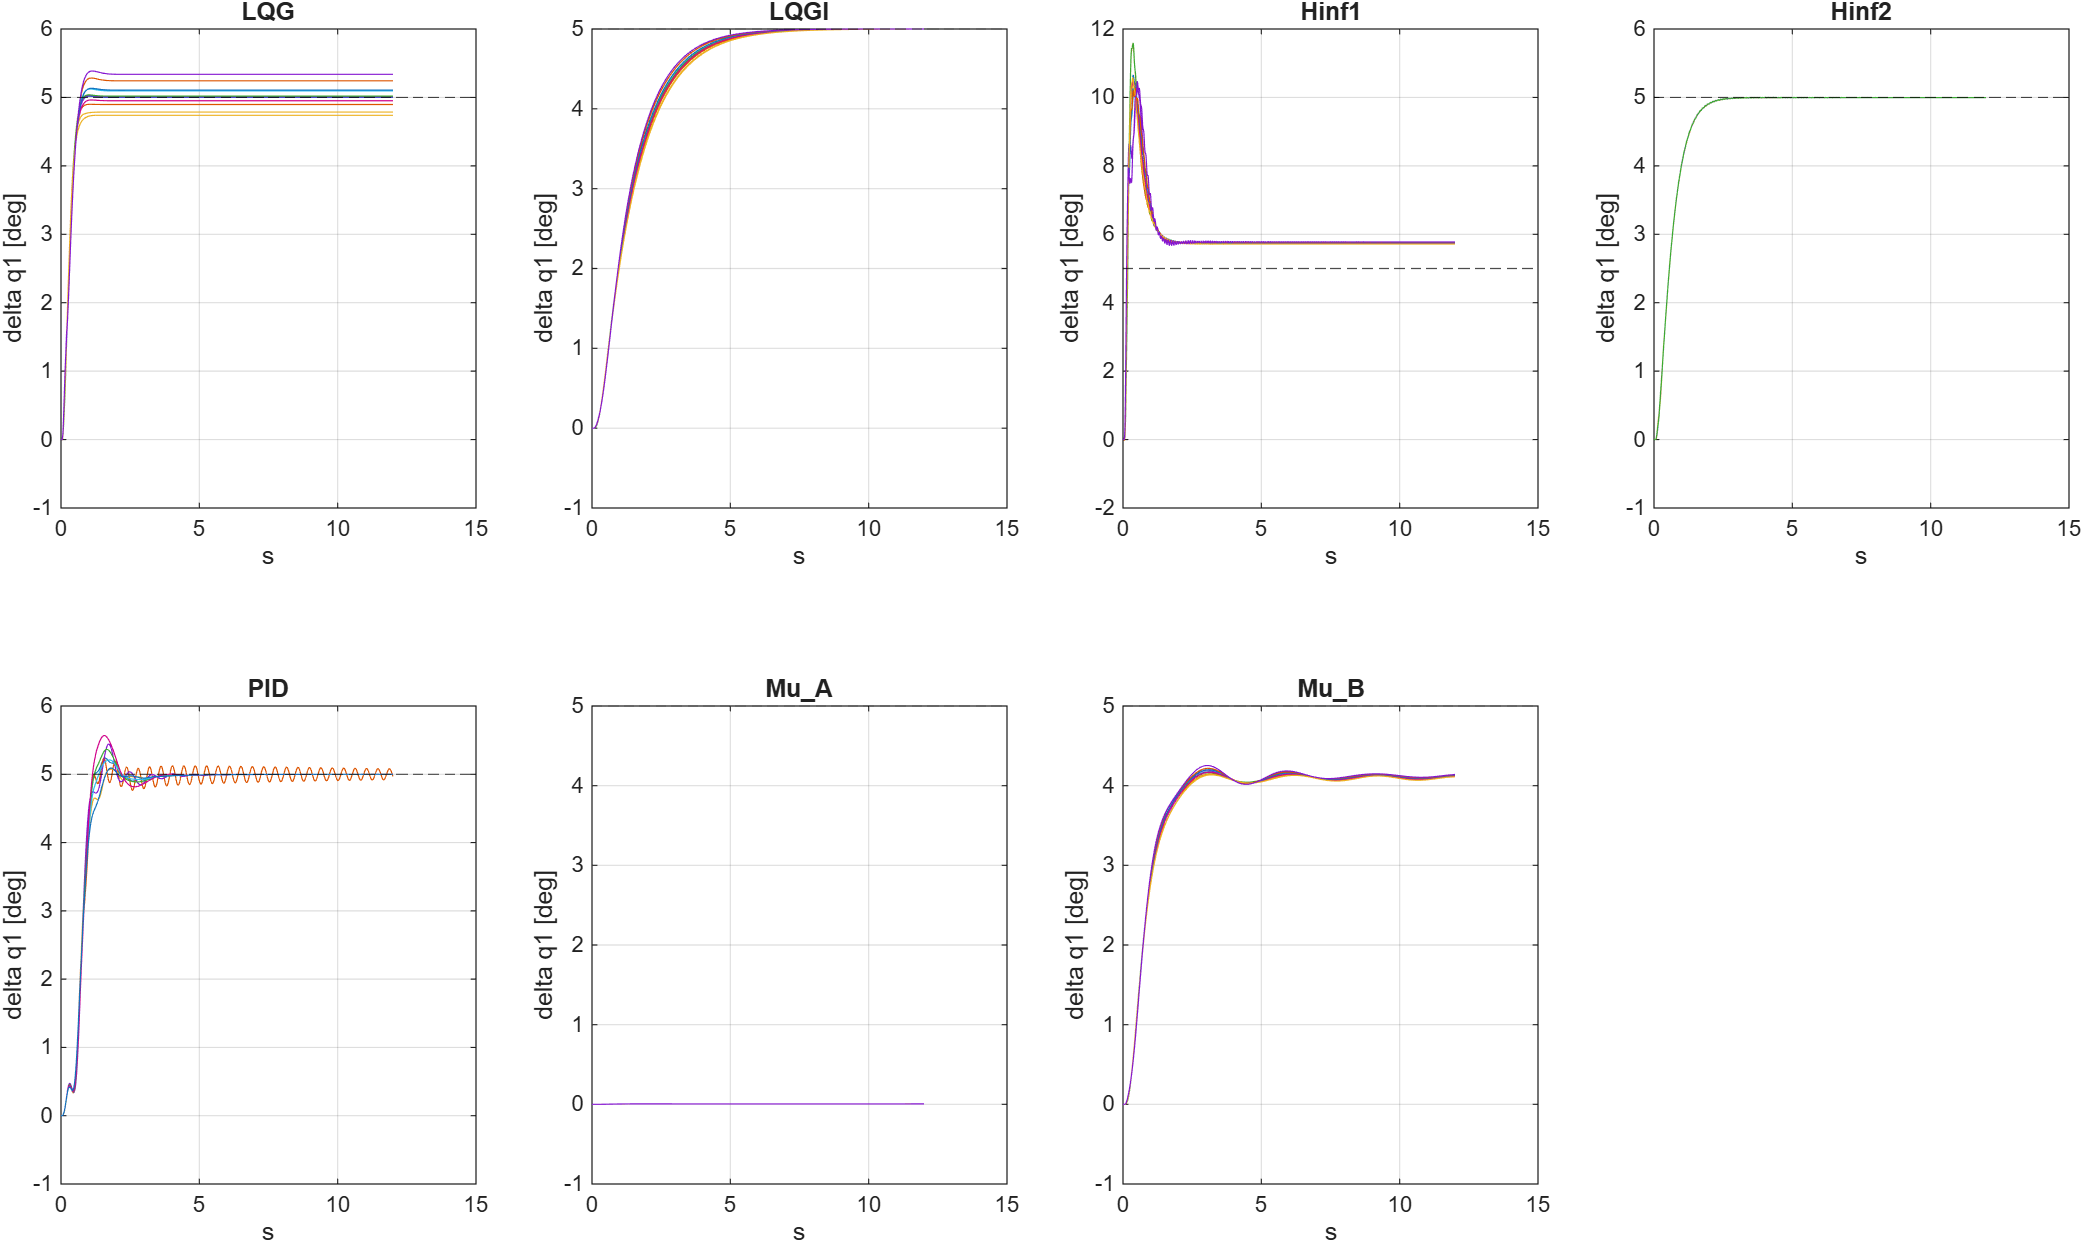
\includegraphics[width=.95\linewidth,height=.34\textheight,keepaspectratio]{figures/definitiva/dieci_impianti.png}
\caption{Gradino di $5^\circ$ al primo giunto. Le curve mostrano
il nominale e i campioni stabili. Il numero di curve di Hinf2 è
ridotto per via delle instabilità registrate in tabella.}
\label{fig:dieci-impianti}
\end{figure}

\section{Rigetto di coppia sui campioni stabili}
Con riferimento nullo applichiamo 0.5 N\,m a un link alla volta.
Il tempo di recupero misura il rientro di entrambi i giunti entro
$0.5^\circ$ dall'equilibrio per il resto della prova. In tabella,
$\infty$ indica rientro mancato entro l'orizzonte di 12 s.

\begin{table}[htbp]\centering\small
\setlength{\tabcolsep}{4pt}
\begin{tabular}{lrrr}\toprule
Controllore & Picco $q_d$ [$^\circ$] & Recupero nom. [s] & Recupero max [s]\\\midrule
LQG & \num{8.84} & $\infty$ & $\infty$\\
LQGI & \num{7.27} & \num{3.48} & \num{3.562}\\
Hinf1 & \num{14.3} & $\infty$ & $\infty$\\
Hinf2 & \num{2.1} & \num{0.346} & \num{0.658}\\
PID & \num{12} & \num{2.95} & \num{3.08}\\
Mu\_A & \num{6.12} & $\infty$ & $\infty$\\
Mu\_B & \num{6.8} & $\infty$ & $\infty$\\
\bottomrule\end{tabular}
\caption{Coppie link separate: peggiore asse nominale e massimo fra campioni stabili. Infinito indica mancato rientro entro 0.5 gradi nell'orizzonte di 12 s.}
\end{table}


Nel peggiore dei dieci casi LQGI rientra in circa 3.56 s,
mentre LQG manca il rientro già nel nominale. Hinf2
rientra in meno di un secondo nell'unico campione stabile.
Il picco di posizione e lo sforzo di comando completano
la lettura dei tempi di recupero.

\paragraph*{Portata della verifica.}
Dieci successi sono un riscontro empirico, mentre anche un solo
campione instabile esclude la garanzia di stabilità su A.
La $\mu$-analysis valuta la famiglia lineare dichiarata, incluse
dinamiche di B senza un corrispondente drive fisico della campagna.
Per valutare insieme variazioni parametriche e rumore encoder
servirebbe una campagna abbinata.
\FloatBarrier
